\section{Ping Pong Tutorial (Java and C)}
\label{sec:ping_pong_tutorial}

\subsection{Scope}

This tutorial describes how to create a simple hierarchical actor system of actors communicating via ports and bindings. 
Additionally you will use the Timing Service from the eTrice model library.
This tutorial can be done for the target languages Java or C.
For the Ping Pong scenario we want to create a model with a sender and a reveiver of a message. The receiver has to wait for the ping message from the sender, wait for a second and respond with a pong message.

The resulting Message Sequence Chart (MSC) at the ende of this tutorial should look like this:

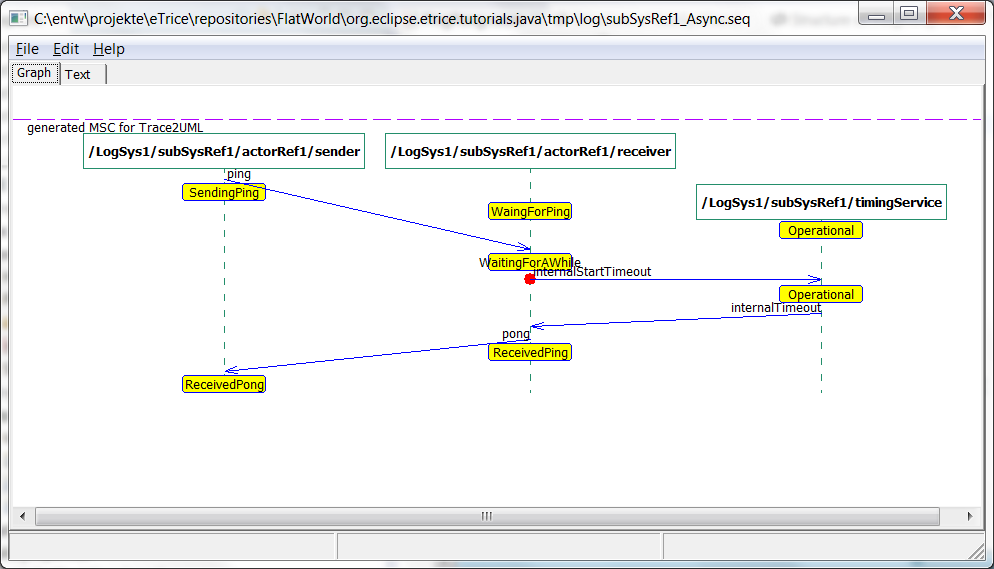
\includegraphics[width=0.8\textwidth]{images/017-01-MSC.png}
% !images/017-01-MSC.png!

We will take this MSC as specification for the desired behavior.

You will perform the following steps:

\begin{enumerate}
\item create a new model from scratch
\item define a protocol
\item create an actor structure
\item create finite state machines
\item use the predefined \textit{TimingService}
\item build and run the model
\item open the message sequence chart
\end{enumerate}

\subsection{Create a new model from scratch}

Create a new \eTrice{} project according to \textit{HelloWorld for Java or C} and name it \textit{PingPong}.

Your \emph{ROOM} model should look like this:

\begin{lstlisting}[language=ROOM]
RoomModel PingPong_Model {
	LogicalSystem LogSys1 {
		SubSystemRef subSysRef1:SubSysClass1 
	}
	SubSystemClass SubSysClass1 {
		ActorRef actorRef1:PingPongTop 
		LogicalThread defaultThread
	}
	ActorClass PingPongTop {
	}
}
\end{lstlisting}

\subsection{Create a new protocol}

First we define a protocol for the communication between the Sender and the Receiver. From the specification MSC above we can derive that the Sender sends a \emph{ping} message to the receiver and the receiver responds with a \emph{pong} message. 

In \emph{ROOM} the \emph{ProtocolClass} specifies interfaces. In this case we go for an asynchronous, bidirectional messaging interface (eventdriven) which is the standard communication type for a \emph{ProtocolClass}.
With the help of \textit{Content Assist} (Ctrl+Space) we create a \textit{ProtocolClass} and name it 
\textit{PingPongProtocol}.
Inside the brackets use the \textit{Content Assist}  to create two incoming messages called 
\textit{ping} and \textit{pong}.

The resulting code should look like this:

\begin{lstlisting}[language=ROOM]
	ProtocolClass PingPongProtocol {
		incoming {
			Message ping()
		}
		outgoing {
			Message pong()
		}
	} 
\end{lstlisting}

With \emph{Ctrl-Shift+F} or selecting \textit{Format} from the context menu you can format the \emph{ROOM} model. Note that 
the new \textit{ProtocolClass} is displayed in the outline view.

\subsection{Create the Actor Structure}
\subsubsection{Add two additional actor classes}

Position the cursor outside any class definition and call the \textit{Content Assist} with \emph{Ctrl+Space}.
Select \textit{ActorClass - actor class skeleton or ActorClass} and name the ActorClass \textit{Sender}.

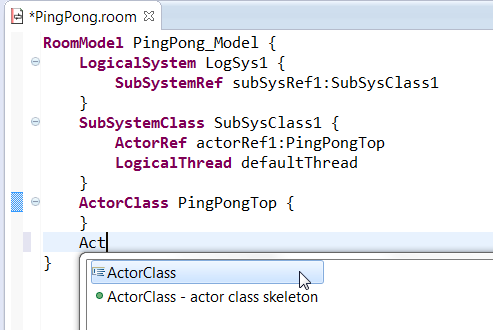
\includegraphics[width=0.6\textwidth]{images/017-02-content-assist.png}
% !images/017-02-content-assist.png!

Repeat the described procedure and name the new actor \textit{Receiver}.

With Ctrl+Shift+F you can format your textual model. 

The Result:

\begin{lstlisting}[language=ROOM]
RoomModel PingPong_Model {

	LogicalSystem LogSys1 {
		SubSystemRef subSysRef1: SubSysClass1
	}

	SubSystemClass SubSysClass1 {
		ActorRef actorRef1: PingPongTop
		LogicalThread defaultThread
	}

	ActorClass PingPongTop { }

	ActorClass Sender { }

	ActorClass Receiver { }

}
\end{lstlisting}

You can should also see the new \emph{ActorClass}es in the outline view.

\subsubsection{Add ports to the actors}

To open the graphical structure editor, right click \textit{Receiver} in the Outline View and select \textit{Edit Structure}. Drag and Drop an 
\textit{Interface Port} from the \emph{Palette} to the border of the \textit{Receiver} actor. Note that an \emph{Interface Port} can only be placed on the border of the actor. Name the port \textit{sender} and select \textit{PingPongProtocol} as Protocol from the drop down list. The checkboxes \textit{Conjugated} and \textit{Is Relay Port} stay unchecked. Click \textit{ok}. The 
resulting structure should look like this:

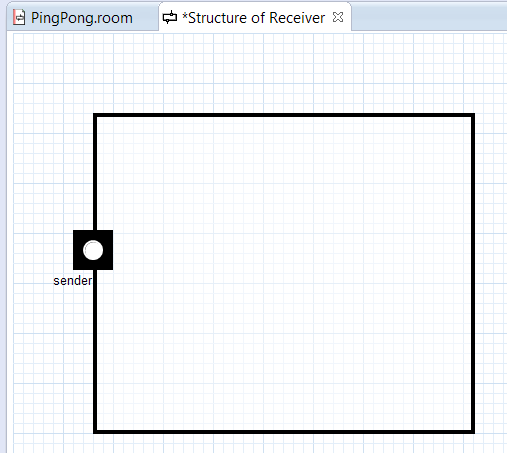
\includegraphics[width=0.6\textwidth]{images/017-04-Port-for-Actor-Receiver.png}
% !images/017-04-Port-for-Actor-Receiver.png!

Repeat the steps above for the \textit{sender}. Create a port named \emph{receiver} with the same \emph{Protocol} and make it \emph{Conjugated}.

Keep in mind that the protocol defines \textit{ping} as incoming message and \textit{pong} as outgoing message. 
\textit{Receiver} receives \emph{ping} and sends \emph{pong}. Therefore the \textit{Receiver}s port must be a 
regular port. The \textit{Sender} has to send \textit{ping} and receive \textit{pong}. Therefore the \textit{Sender}s port must be a conjugated port.

\subsubsection{Build hierarchical actor structure}

Now we want to add the new actors to the structure of \emph{ActorClass} \emph{PingPongTop}.

From the outline view right click \textit{PingPongTop} and select \textit{Edit Structure}. Remember that you can only see the outline view if the textual editor with the .room file is active.

Drag and Drop an \textit{ActorRef} inside the \textit{PingPongTop} actor. Name it \textit{sender}. From the actor class drop down list select \textit{Sender}. Do the same for \textit{Receiver}. Connect the ports 
via the binding tool int the \emph{Palette}. The resulting structure should look like this:

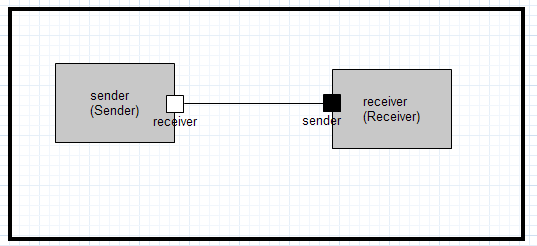
\includegraphics[width=0.8\textwidth]{images/017-03-PingPongTop-Structure.png}
% !images/017-03-PingPongTop-Structure.png!

We have build the structure of a hierarchical actor system with two actors that send each other messages.

\subsubsection{Import the Timing Service}

In order to implement the waiting time of the \emph{Receiver} we need a timing service. The timing service is provided by the model library and must be imported before it can be used in your model.

\begin{figure}[ht]
\begin{minipage}[t]{0.50\linewidth}
\begin{mdframed}
	\textbf{room model for Java}
	\newline
\begin{lstlisting}[language=ROOM]
RoomModel PingPong_Model {

	import room.basic.service.timing.* from "../../org.eclipse.etrice.modellib.java/model/TimingService.room"
	(...)
\end{lstlisting}
\end{mdframed}
\end{minipage}
\hspace{0.1cm}
\begin{minipage}[t]{0.50\linewidth}
\begin{mdframed}
	\textbf{room model for C}
	\newline
\begin{lstlisting}[language=ROOM]
RoomModel PingPong_Model {

	import room.basic.service.timing.* from "../../org.eclipse.etrice.modellib.c/model/TimingService.room"
	(...)
\end{lstlisting}
\end{mdframed}
\end{minipage}
\end{figure}

This is the first time you use an element from the modellib. Make sure that your Java Build Path or the settings for your C compiler are configured to use the modellib. Otherwise the generated code can not be built.

\begin{figure}[ht]
\begin{minipage}[t]{0.50\linewidth}
\begin{mdframed}
	\textbf{build settings for Java}
	\newline
Right click the project \textit{PingPong} and select \emph{Properties -> Java Build Path -> Projects} . Add the project \emph{org.eclipse.etrice.modellib.java} .
  
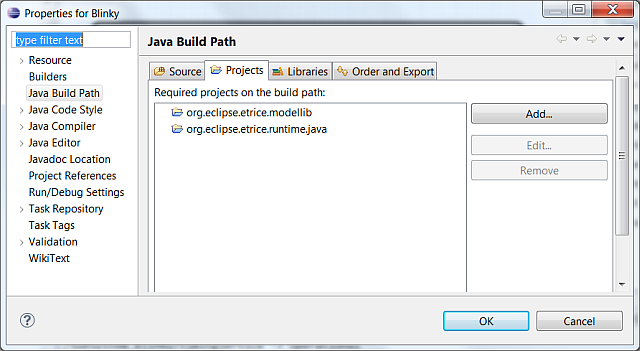
\includegraphics[width=0.8\textwidth]{images/020-Blinky16.png}
% !images/020-Blinky16.png! 

\end{mdframed}
\end{minipage}
\hspace{0.1cm}
\begin{minipage}[t]{0.50\linewidth}
\begin{mdframed}
	\textbf{build settings for C}
	\newline

Right click the project \textit{PingPong} and select \emph{Properties -> C/C++ Build -> Settings -> Includes}. Add the include path \emph{org.eclipse.etrice.modellib.c/src-gen} to the list.

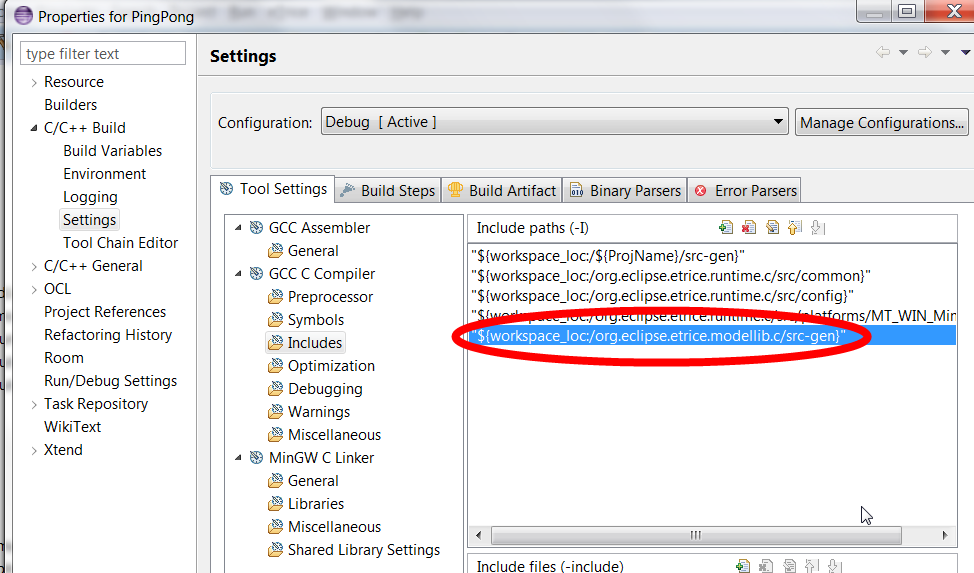
\includegraphics[width=0.8\textwidth]{images/017-06-Settings-for-C-Includes.png}
% !images/017-06-Settings-for-C-Includes.png! 

Select \emph{Properties -> C/C++ Build -> Settings -> Libraries}. Add the library \emph{org.eclipse.etrice.modellib.c} and the library path 
\emph{org.eclipse.etrice.modellib.c/MinGWDebug} to the lists. For Posix the path will be \emph{org.eclipse.etrice.modellib.c/PosixDebug}.
	
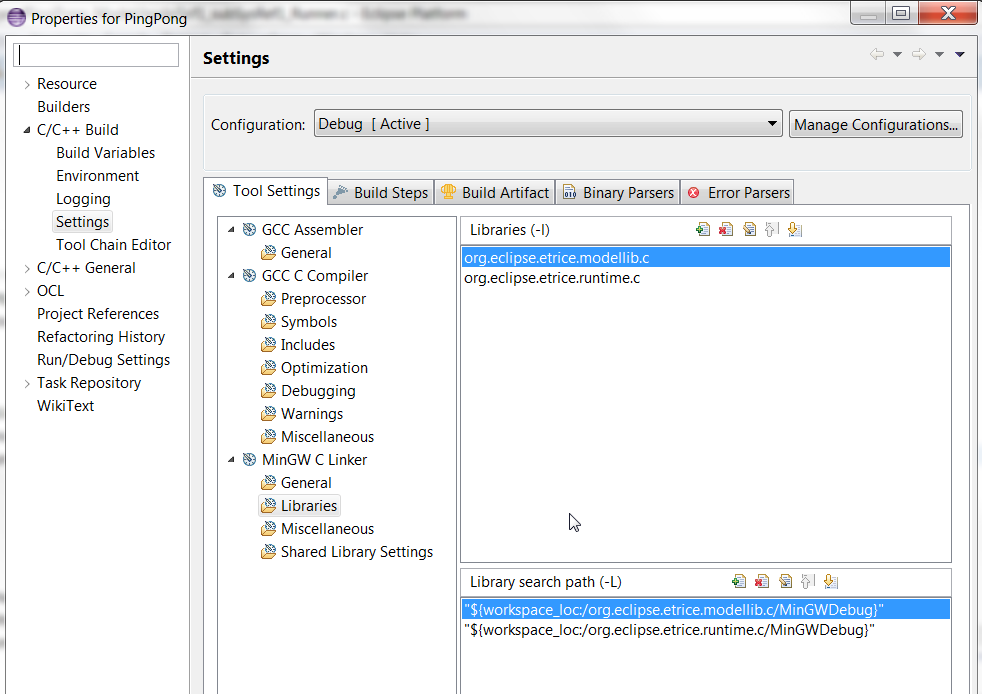
\includegraphics[width=0.8\textwidth]{images/017-07-Settings-for-C-Libraries.png}
% !images/017-07-Settings-for-C-Libraries.png! 

\end{mdframed}
\end{minipage}
\end{figure}

Now the imported library can be used within your model and we will add the actor with the timing service to our model.

Right click the \emph{SubSystemClass} \emph{SubSysClass1} in the outline view and select \textit{Edit Structure}. The \emph{ActorClass} \emph{PingPongTop} is already referenced in the subsystem as \textit{actorRef1}. Drag and 
Drop an \textit{ActorRef} into the structure of \emph{SubSysClass1} and name it \textit{timingService}. From the actor class drop down list select \textit{room.basic.service.timing.ATimingService}. Draw a 
\textit{LayerConnection} from \textit{actorRef1} to the service provision point (\emph{SPP}) of the 
\textit{timingService}. The resulting structure should look like this:

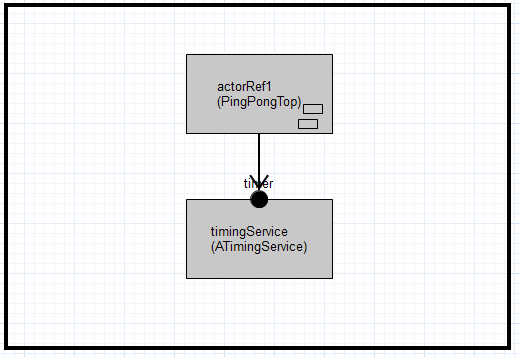
\includegraphics[width=0.8\textwidth]{images/017-08-SubSystem-with-timing-service.png}
% !017-08-SubSystem-with-timing-service.png! 

The layer connection between an \emph{ActorRef} and a \emph{SPP} enables the use of service access points (\emph{SAP}) for the service provided by the \emph{SPP}, in this case the timing service. \emph{SAP}s and \emph{SPP}s are ports with a different kind of connection. Every \emph{SAP} of the type \emph{PTimer} inside actorRef1 is now connected automatically by the code generator with the \emph{SPP} of the \emph{timingService}.

The current version of \eTrice{} does not provide a graphical element for a service access point (SAP). 
Therefore the SAPs to access the timing service must be added in the .room file. Open the 
\textit{PingPong.room} file and navigate to the \textit{Receiver} actor. Add the SAP for the protocol \emph{PTimer} to the structure of the actor:

\begin{lstlisting}[language=ROOM]
	ActorClass Receiver {
		Interface {
			Port sender: PingPongProtocol
		}
		Structure {
			external Port sender
			SAP timing : PTimer
		}
	}
\end{lstlisting}

Now the \emph{Receiver} can use the timing service.

\subsubsection{Inspect the Actor Structure}
Before we start with the implementation of the behavior we will have a short look at the instance tree of the application we built so far:

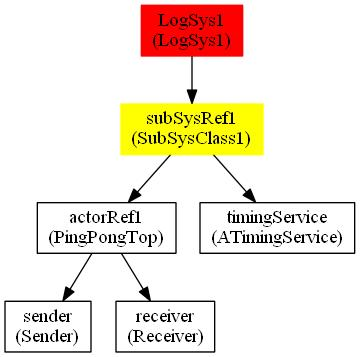
\includegraphics[width=0.4\textwidth]{images/017-09-PingPong_InstanceTree.jpg}
% !017-09-PingPong_InstanceTree.jpg! 

For each instance you can see the names of the \emph{ActorRef}s and in brackets the names of the \emph{ActorClass}es. Starting at the subsystem level this instance tree will be implemented by the code generator. The subsystem will be implemented as process in Linux or Windows.


\subsection{Implement the Behavior}

We will implement two finite state machines (\emph{FSM}s) to  define the event driven behavior of the actors  \emph{Sender} and \emph{Receiver}.

Before you start with the implementation, have a look at the MSC with the specification of the behavior.

Lets start with the \emph{Sender}. Right click to \emph{Sender} in the outline view or the structure editor and select \emph{Edit Behavior}.
Drag and Drop the \textit{Initial Point} and two \textit{States} into the top state. Name the states 
\textit{SendingPing} and \textit{ReceivedPong}. 
Use the \textit{Transition} tool to draw transitions from \textit{init} to \textit{SendingPing} and from \textit{SendingPing} to \textit{ReceivedPong}.
When you draw a transition, the Dialog \emph{Edit Transition} opens. Here you can specify the trigger event and the action code for each transition. Note that the initial transition does not have a trigger event.
The transition dialog for the Transition from \textit{SendingPing} to \textit{ReceivedPong} should look like this:

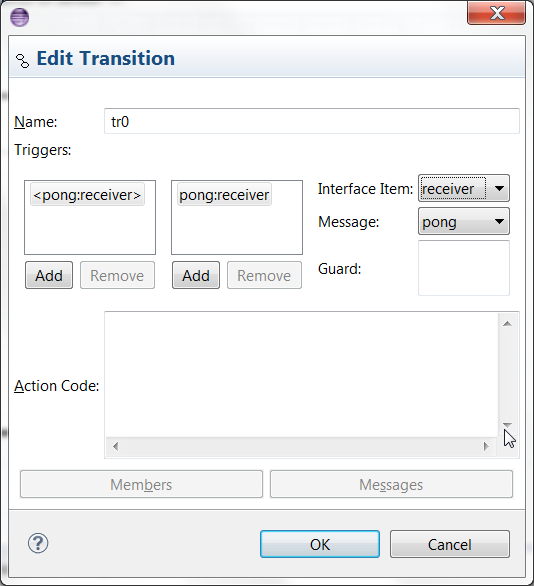
\includegraphics[width=0.6\textwidth]{images/017-10-Edit-Transition.png}
% !images/017-10-Edit-Transition.png! 

The transition will now be triggered by an incoming message \emph{ping} at the port \emph{receiver}.

Now we open the dialog \emph{Edit State} of the state \textit{SendingPing} by right clicking the state and selecting \emph{Edit State} from the menu.
We want to send the message \emph{ping} in the entry code of this state.
The defined ports will be generated as a member attribute of the actor class from type of the attached 
protocol. To send a message you must state \textit{port.message(param);}. In this example 
\textit{receiver.ping();} sends the \textit{ping} message via the \textit{receiver} port. You can also use the Button \emph{Messages} to select the message from the list of available ports and their available messages.
Assuming that the actor \textit{Receiver} is connected to this port, the message will be sent there.

The FSM of \emph{Sender} should now look like this:

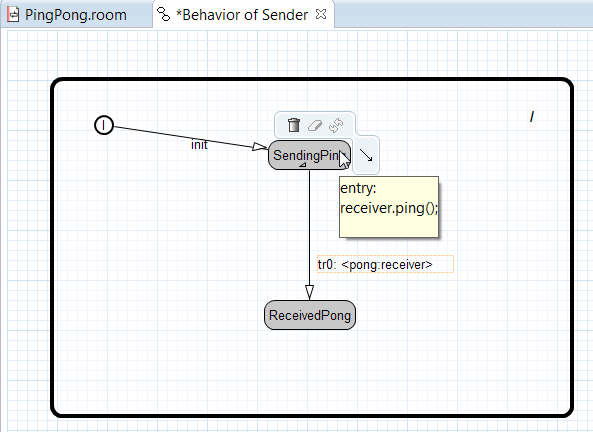
\includegraphics[width=0.8\textwidth]{images/017-11-FSM-Sender.png}
% !images/017-11-FSM-Sender.png!

Now we implement the FSM of the \emph{ActorClass} \emph{Receiver}.

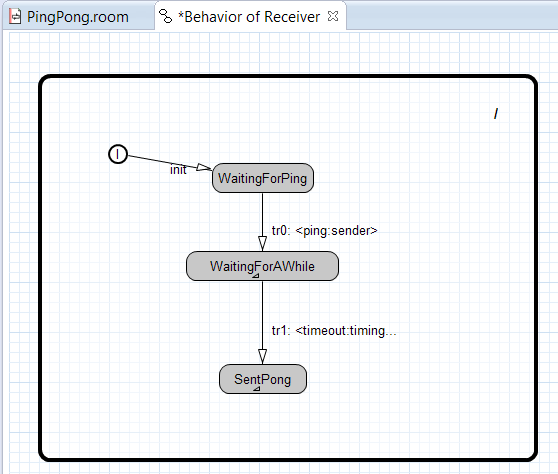
\includegraphics[width=0.8\textwidth]{images/017-12-FSM-Receiver.png}
% !images/017-12-FSM-Receiver.png!

In the entry code of the state \emph{WaitingForAWhile} we start the timeout: 

\begin{verbatim}
timing.startTimeout(1000);
\end{verbatim}

In the entry code of the state \emph{SentPong} we send the message \emph{pong} back to the \emph{Sender}: 

\begin{verbatim}
sender.pong();
\end{verbatim}

Save the diagram and inspect the \emph{PingPong.room} file. The \emph{Receiver} should look like this:

\begin{lstlisting}[language=ROOM]
	ActorClass Receiver {
		Interface {
			Port sender: PingPongProtocol
		}
		Structure {
			external Port sender
			SAP timing : PTimer
		}
		Behavior {
			StateMachine {
				Transition init: initial -> WaitingForPing { }
				Transition tr0: WaitingForPing -> WaitingForAWhile {
					triggers {
						<ping: sender>
					}
				}
				Transition tr1: WaitingForAWhile -> SentPong {
					triggers {
						<timeout: timing>
					}
				}
				State WaitingForPing
				State SentPong {
					entry {
						"sender.pong();"
					}
				}
				State WaitingForAWhile {
					entry {
						"timing.startTimeout(1000);"
					}
				}
			}
		}
	}
\end{lstlisting}

The PingPong model is done now. You can generate, compile and run it as described in \emph{Hello World for C} or \emph{Hello World for Java}. The generated MSC in tmp/log should show the same MSC we used to specify the behavior at the beginning of this tutorial.

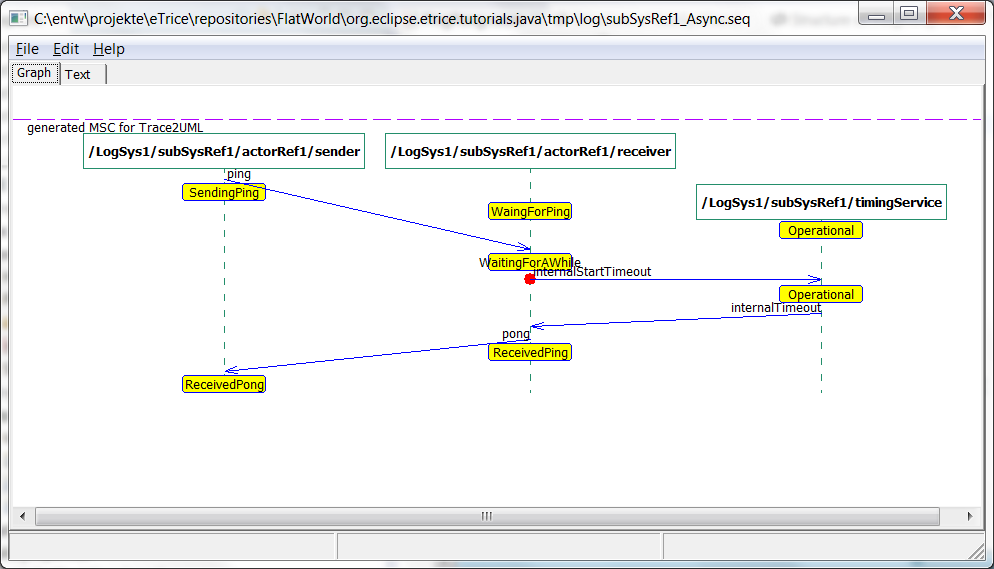
\includegraphics[width=0.8\textwidth]{images/017-01-MSC.png}
% !images/017-01-MSC.png!

Please note that the timeout messages startTimeout and timeout might vary depending on the target language and are not displayed completely correct in the current version (red dot). The MSC logger will be extended to handle this correct in the next version.

\subsection{Summary}

Within this tutorial you have learned how to create a FSM with transitions triggered by incoming messages. You have used entry code to send messages and have used the timing service from the model library. You are now familiar with the basic features of \eTrice{}. Further tutorials and examples will take this knowledge as a precondition.
